
\section{Stokes drift}
The displacements of fluid parcels caused by waves is dominated by the periodic oscillations  $\widetilde{\mathbf \xi}_h$ and
$\widetilde{\xi}_3$ derived in chapter \ref{ch1b} for linear waves. For many application this first approximation may not be sufficient.
Let us examine what has been neglected. 
To be exact, the position $\left({\mathbf x}(t),z(t)\right)$
of a fluid parcel is the sum of its velocities at the successive positions \citep[e.g.][p. 43]{Phillips1977},
\begin{equation}
    \left({\mathbf x}(t),z(t)\right)= \left({\mathbf x}(0),z(0)\right)
    +\int_0^t \left(\mathbf{u}\left({\mathbf x}(t^\prime),z(t^\prime),t^\prime\right),w\left({\mathbf x}(t^\prime),z(t^\prime),t^\prime\right)\right) {\mathrm
    d}t^\prime.
\end{equation}

To the first order in steepness $\varepsilon=ka$, the velocity equals the velocity at the initial position, 
\begin{equation}
 \left(\mathbf{u}\left({\mathbf
x}(t^\prime),z(t^\prime),t^\prime\right),w\left({\mathbf
x}(t^\prime),z(t^\prime),t^\prime\right)\right)
\simeq \left(\mathbf{u}\left({\mathbf
x}(0),z(0),t^\prime\right),w\left({\mathbf
x}(0),z(0),t^\prime\right)\right).
\end{equation}
Integrating in time this gives a periodic motion, 
$\left({\mathbf x}(t),z(t)\right)=\left({\mathbf
x}(0),z(0)\right)+(\xi_h,\xi_3)$ as given by eqs.
(\ref{xi1})--(\ref{xi3}). 


%%%%%%%%%%%%%%%%%%%%%%%%%%%%%%%%%%%%%%%%%%%%%%%%%%%%%%%%%%%%%%%%%%%%%%%%%%%%%
\begin{figure}[htb]
\centerline{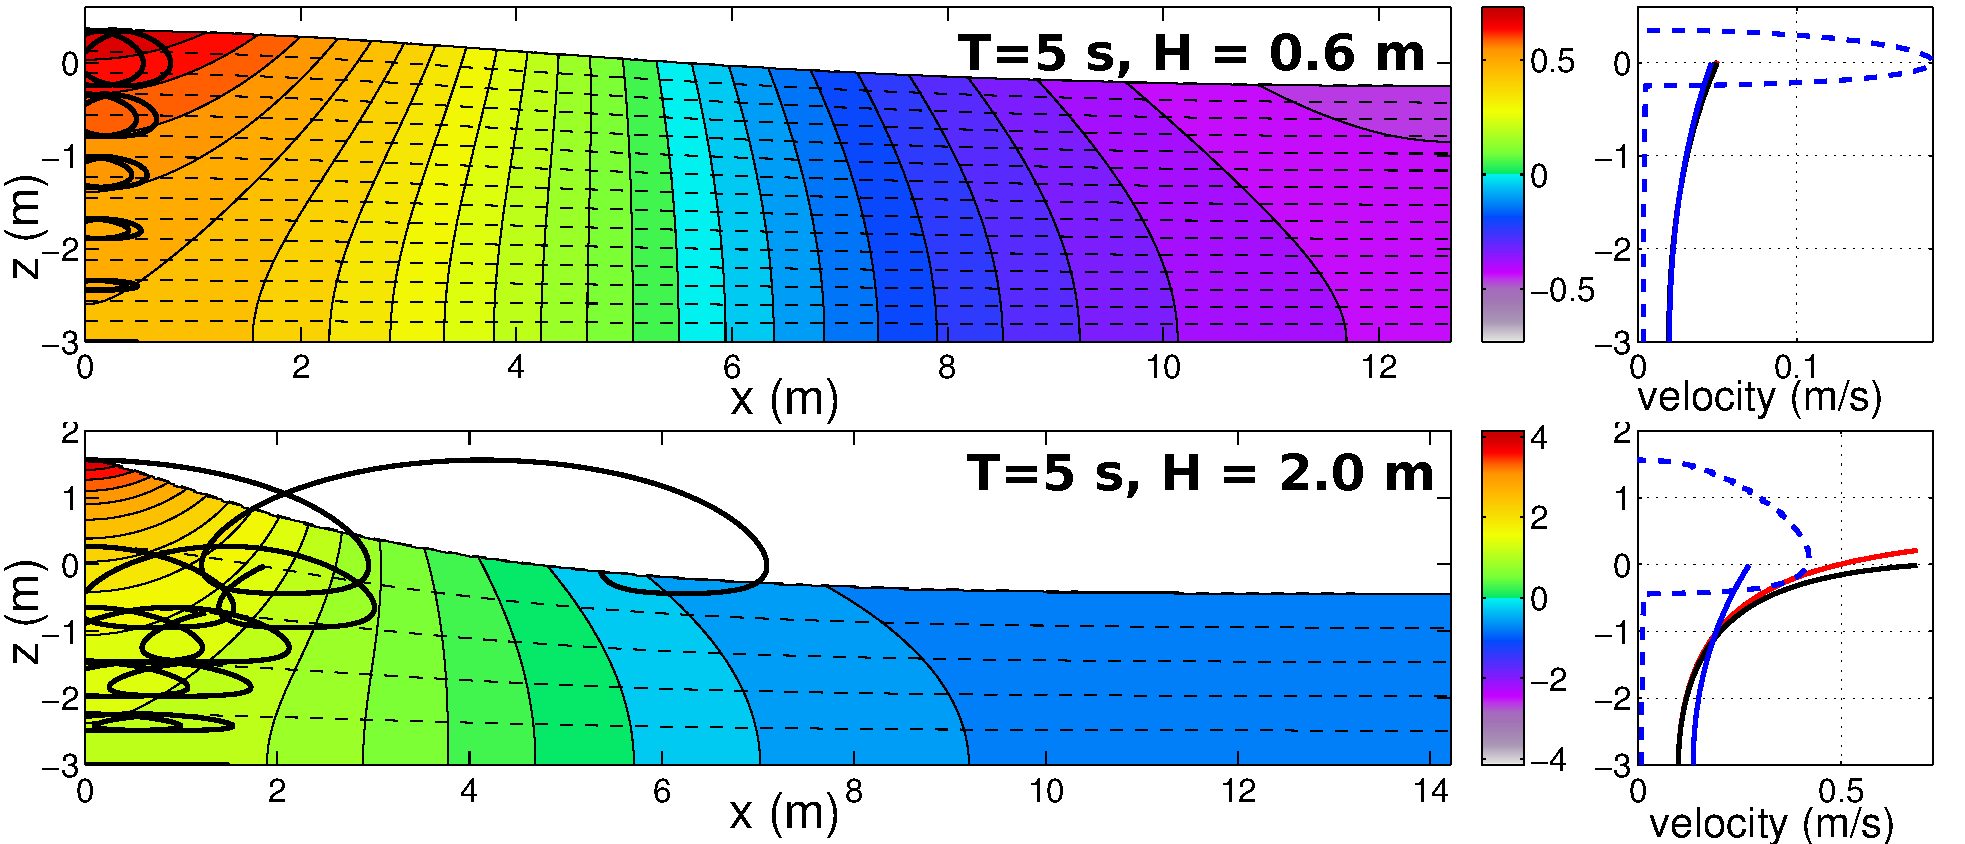
\includegraphics[width=0.9\textwidth]{FIGS_CH_MOMENTUM/Drift_lin_nonlin.pdf}}
%\vspace{3.64in}
  \caption{Left: Horizontal velocity field at $t=0$ and particle trajectories integrated over 2 Eulerian periods. 
Solid lines are isotachs and dashed lines are streamlines in the frame of reference moving with the wave phase speed. Right: vertical profile of Eulerian mean water velocity (dashed, velocity 
is set to zero in the air for computing the average), Generalized Lagrangian mean (red), Lagrangian mean (black) and Lagrangian mean from the linear 
approximation (blue). Both top and bottom panels are computed with streamfunction theory to 80th order \citep{Dalrymple1974}. Non-linear terms are only significant in the bottom case.}
\label{fig:drift_stream}
\end{figure}
%%%%%%%%%%%%%%%%%%%%%%%%%%%%%%%%%%%%%%%%%%%%%%%%%%%%%%%%%%%%%%%%%%%%%%%%%%%%%
However, the exact calculation (figure \ref{fig:drift_stream}) shows that the motion is not periodic. This is because the velocity varies over the displacement 
distance. That variation introduces a correction of the position that is of second order 
in the wave amplitude. This is given by the following Taylor expansion 
\begin{eqnarray}
    \mathbf{u}\left({\mathbf x}(t^\prime),z(t^\prime),t^\prime\right) & =&
    \mathbf{u}\left({\mathbf x}(0),z(0),t^\prime\right) \nonumber\\
   && +  \mathbf{u}_2\left({\mathbf x}(0),z(0),t^\prime\right)  \nonumber\\
    &&+ \xi_h(t')\bcdot \bnabla \mathbf{u}\left(\xi_h(0),\xi_3(0),t^\prime\right)
    +\xi_3(t') \frac{\partial}{\partial z} \mathbf{u}\left(\xi_h(0),\xi_3(0),t^\prime\right)
    + O(\varepsilon^3),\label{eq:Stokes_drift_Taylor}
    \end{eqnarray}
where $\mathbf{u}_2$  is the gradient of the second order potential $\phi_2$,
    which comes in the solution of non-linear wave equation (\ref{surface comb}). That term can be rather complex to compute, and it is 
done in chapter \ref{chnl2}. However, we do not need to worry about that term because the average over time of $\mathbf{u}_2$  is zero. 
We will thus only consider the last two terms which are given by products of linear terms. 

    First of all $\xi_h(t)$ is 90 degrees out of phase with $\mathbf{u}$, and 
    $\bnabla \mathbf{u}$ is also 90 degrees out of phase with   $\mathbf{u}$. 
    Hence   $\xi_h(t)$  and $\bnabla \mathbf{u}$  are in phase and their product has 
a non-zero average, $\kb \sigma a^2 \cosh^2(kz+kh)/[2 \sinh^2(kD)]$. Physically this corresponds to the fact that the orbital velocity at the crest 
is in the same direction as the crest motion, hence particles ride with the crest longer than they stay in the trough where particles move opposite to the 
wave propagation.
  Likewise, $\xi_3$  is in phase with ${\partial \mathbf{u}}/{\partial z}$, which corresponds to the fact that the horizontal velocity increases vertically, 
and thus a particle goes forward faster when it is up compared to when it is down. 
That other product gives also a non-zero average, $\kb \sigma a^2 \sinh^2(kz+kh)/[2 \sinh^2(kD)]$. These two effects add up to give  the Stokes drift, defined as
\begin{equation}
    {\mathbf U}_s\equiv \frac{1}{T_L}\int_0^T \mathbf{u}\left({\mathbf x}(t^\prime),z(t^\prime),t^\prime\right) \mathrm d t^\prime 
= \sigma \kb a^2 \frac{\cosh(2kz+2kh)}{2\sinh^2(kD)} (1+O(\varepsilon)),
\end{equation}
where $T_L$ is the Lagrangian period, namely the time it takes for a parcel starting from a crest to loop to the next crest.
The bottom panel in figure  \ref{fig:drift_stream} clearly shows that the Lagrangian period is longer than the Eulerian period: after two Eulerian period 
the particles that started at the crest are not yet back to the crest, because they have moved forward ahead of the next crest. 

In deep water ($kD \gg 1$), $U_s$ goes to
\begin{equation}
    {\mathbf U}_s=\sigma \kb a^2 \exp(2kz).\label{eq:Us_mono_deep}
\end{equation} 

This speed $U_s$ is the average drift speed of a water parcel and it is directed in the direction of wave propagation. It 
is a mean Lagrangian velocity. Hence the parcel displacement is not exactly periodic and the parcels move forward (figure \ref{fig:puvdrift}). This 
drift velocity decreases strongly with depth, in deep water this decrease is twice as fast as the orbital velocity, as shown on figure  \ref{fig:puvdrift}.

First of all, it should be emphasized that we have computed a second order drift from a linear wave field. 
The top-right  panel in figure \ref{fig:drift_stream} clearly shows that for a nearly linear wave the Stokes drift is dominated by the 
contribution of linear wave field (blue profile). There is a widely held misconception that Stokes drift is a property of non-linear waves. 
This is wrong.  In fact, the Stokes drift is a quadratic property, just like the wave energy. Linear waves have a Stokes drift, just like 
they have an energy. 


This correspondence between Stokes drift and energy is a very profound physical property \citep{Andrews&McIntyre1978b}. 
The Stokes drift computed here is the pseudo-momentum of the wave field. When integrated over the vertical it is 
\begin{equation}
    {\mathbf M}^w=\rho_w \int_{-h}^0 {\mathbf U}_s {\mathrm d} z =
    \frac{\cosh (kD)}{2 \sinh (kD)} \rho_w \sigma a^2 = \rho_w g
    \frac{a^2}{2C} =  \frac{E_t}{C} \label{eq:momentum-energy}
\end{equation}
with $E_t$ the wave energy per unit surface. Eq. (\ref{eq:momentum-energy}) is a very general result in physics for all types of waves. 
It is the same result as the momentum of a photon $p=E/c$, where $c$ is the speed of light. For non-linear waves of finite 
amplitude, the exact relationship is ${\mathbf M}^w=2 {E_c}/{C}$, where $E_c$ is the mean kinetic energy per unit surface \citep[][
see chapter \ref{ch_nonlin_per}]{Longuet-Higgins1984}.

Finally, this transport can also be computed from the Eulerian velocity, 
integrated from the bottom to the crest level, 
\begin{equation}
    {\mathbf M}^w=\rho_w \left< \int_{-h}^\zeta {\mathbf u} {\mathrm d} z \right> =
    \int_{-a}^a \left< \rho {\mathbf u} \right> {\mathrm d} z
\end{equation}
These two estimates of the transport correspond to the two different views of the Stokes drift. 
In the Eulerian point of view, the mass transport only happens between the crests and the troughs, with a profile that 
is a parabola for linear waves. In the Lagrangian point of view the drift happens over the entire water column (figure \ref{Eul_Lag_drift}).
%%%%%%%%%%%%%%%%%%%%%%%%%%%%%%%%%%%%%%%%%%%%%%%%%%%%%%%%%%%%%%%%%%%%%%%%%%%%%
\begin{figure}
\centerline{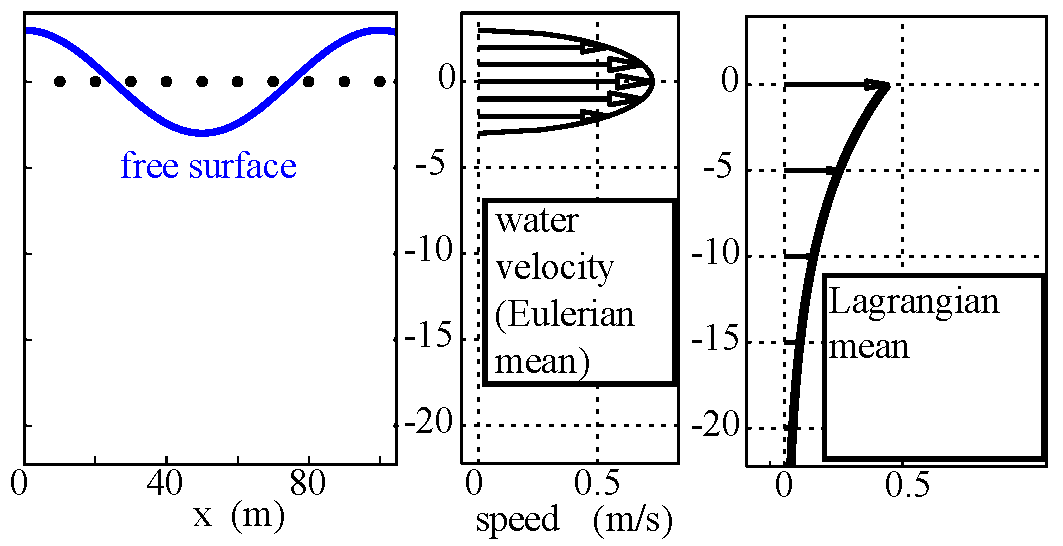
\includegraphics[width=0.8\textwidth]{FIGS_CH_MOMENTUM/Eul_Lag_drift_en.pdf}}
%\vspace{3.64in}
  \caption{Mass transport from an Eulerian and Lagrangian point of views, computed here 
for an amplitude $a=3$~m, wavelength $L=100$~m in 30~m water depth, using 
linear wave theory.}
\label{Eul_Lag_drift}
\end{figure}
%%%%%%%%%%%%%%%%%%%%%%%%%%%%%%%%%%%%%%%%%%%%%%%%%%%%%%%%%%%%%%%%%%%%%%%%%%%%%

Finally, we also note that there is also a Stokes drift in the air, which is also in the direction of propagation 
and has a profile that decays vertically up, like the profile of Stokes drift in deep water. It is easily 
computed by the same method that was used here in the water. 

\section{The `shear' of the Stokes drift}
Another interesting property of the Stokes drift is that it has a strong vertical shear, in particular in deep water, but also 
for strongly nonlinear waves in shallow water \citep{Miche1944d}. This may seem paradoxical that an irrotational flow, with zero vorticity, has an average with a strong shear. This apparent paradox comes from the fact that the curl operator does 
not commute with the Lagrangian average. Another funny property is that the Lagrangian average of $dw/dx$ is also non-zero, 
although the motion is periodic in $x$ \citep{Ardhuin&Jenkins2006}.

The shear of the Stokes drift also has the very nice property to persist in the presence of strong mixing, because the mixing is usually done by eddies that have time scales longer than the wave period. Hence one should be very careful to apply to the wave motion the eddy viscosity ideas that are usual for currents. Indeed, the assumption that the effect of turbulence is analogous the the molecular viscosity scaled up by a factor 100 or more does not work with waves: if it were the case the waves would dissipate over very short distance and swells would never be recorded from remote storms. 
The `eddy viscosity' idea is thus a very dangerous idea in the presence of oscillations, and turbulence closures should generally be visco-elastic and not just viscous \citep[e.g.][]{Miles1996b}. 

This persistence of the vertical shear of the drift makes the ocean surface boundary layer special and tends to tilt vorticity that is perpendicular to the wind into the wind direction, promoting the generation of rolls aligned in the wind. 
These are known as Langmuir circulations \citep{Langmuir1938}, which is a key component of the ocean mixed layer. 
These properties of the upper ocean will be further discussed in chapter \ref{ch_ioa}.

\section{Random waves and practical estimation}
Although the Stokes drift plays an important role, it is very difficult to measure in the ocean because it requires the measurement of both the Eulerian velocity and the drift at the same place, and drift if usually measured at the surface only with objects that can be also affected by the direct influence of the wind or the radiation stress of the very short waves. Indeed, no object or surfactant drifts exactly like the water surrounding it, and only non-intrusive methods using for example infrared technology \citep{Veron&al.2008} or surface wave dispersion \citep{Laxague&al.2018} can provide unambiguous measurements.

As a result, almost all estimates of the Stokes drift are based on the measurement of the wave spectral properties and the use of linear wave theory because the Stokes drift for a random wave field with no phase-correlations between the wave components is simply derived from eq. (\ref{eq:Stokes_drift_Taylor}), as done by \cite{Kenyon1969}. The horizontal Stokes drift vector is thus,  
\begin{equation}
 (U_S, V_S) = \int_0^{\infty}  2 \sigma  k  \frac{\cosh(2kz+2kh)}{2\sinh^2(kD)} \int_0^{2 \pi} (\cos \theta,\sin \theta)  E(f,\theta) \mathrm{d}\theta \mathrm{d} f.
\end{equation}
The inner integral can be replaced by the moments $a_1$ and $b_1$ that are directly measured by wave buoys (see chapter \ref{ch_anaspec} for details), 
\begin{equation}
 (U_S, V_S) = \int_0^{\infty}   2 \sigma  k  \frac{\cosh(2kz+2kh)}{2\sinh^2(kD)} (a_1(f),b_1(f))  E(f)  \mathrm{d} f.
\end{equation}

The broad directional spectrum at high frequency contributes little to the total surface drift \citep{Peureux&al.2018}. As a result, the vertical profile of the Stokes drift can have a strong shear but weaker than predicted by simple parameterizations such as the one by \cite{Breivik&al.2016}, or when using parametric spectra such as the one by \cite{Elfouhaily&al.1997}.

Finally we note that non-linear effects typically enhance the drift, such as shown in figure \ref{fig:drift_stream}. But there is no published theory giving the expression for nonlinear corrections to the Stokes drift for a random wave spectrum. That can be derived using the surface elevation second order spectrum \citep{Janssen2009,Leckler&al.2015}.

\section{Radiation stresses and the flux of wave momtum \label{section:Sxx}}
Just like the wave energy is radiated by the wave field, the wave momentum is also radiated away. 
Considering monochromatic waves (i.e. with a single period and direction) propagating 
along the $x$-axis, there is a flux of momentum across any surface perpendicular to the propagation direction. By definition, 
there are two ways to move momentum in the $x$ direction, 
\begin{itemize}
 \item by pushing things around: the pressure forces transmit momentum from one water column to the next,
 \item by advecting the momentum density per unit volume $\rho u$ with the velocity $u$.
\end{itemize}

The usual definition of the momentum flux associated to waves, and called the `radiation stress', is the 
flux of momentum when the waves are present minus the flux when waves are absent. It is a strange definition because the interaction of 
waves and currents make it impossible to have the exact same current without the waves, in practice it means 
that we assume the sea level to remain the same and we just set the orbital velocity to zero and the pressure becomes the hydrostatic pressure. 
A more rigorous definition is given in \cite{Andrews&McIntyre1978b}
and discussed in chapter \ref{ch_vaguescourant3D}. Anyway, let us make this thought experiment of  removing the waves, 
 we define the first component of the radiation stresses by a phase average of the wave effects, 
\begin{equation}
    S^{\mathrm{rad}}_{xx}=\overline{ \int_{-h}^\zeta p + \rho_w u^2 \mathrm{d}z }
    -\int_{-h}^{\overline{\zeta}} p_0 + \rho_w \widehat{u}^2   \mathrm{d}z,
\end{equation}
where the second term correspond to the pressure $p_0$ in the absence of waves (but with the same mean sea level) and $\widehat{u}$ is the 
the mean (current) velocity. 

When the waves are present, the pressure is obtained by integrating the vertical component of the 
momentum equation  (we take $v=0$ because waves propagate only along the $x$-axis) 
\begin{equation}
    \int_z^\zeta \left[ \frac{\partial \rho_w w}{\partial t}
                + \frac{\partial \rho_w uw}{\partial x}
                + \frac{\partial\rho_w w^2}{\partial z}
                + \frac{\partial p}{\partial z}
                +\rho_w g\right] {\mathrm d}z=0
\end{equation}
The first term yields
\begin{equation}
    \int_z^\zeta \frac{\partial \rho_w w }{\partial t} {\mathrm d}z
    =\frac{\partial }{\partial t} \int_z^\zeta \rho_w w {\mathrm d}z
    - \rho_w w\left(\zeta\right)\frac{\partial \zeta}{\partial t},
\end{equation}
the second yields, 
\begin{equation}
    \int_z^\zeta \frac{\partial \rho_w uv}{\partial x} {\mathrm d}z
        =\frac{\partial }{\partial x}  \int_z^\zeta \rho_w uw {\mathrm d}z
        -\rho_w u\left(\zeta\right)w\left(\zeta\right)
        \frac{\partial \zeta}{\partial x}
\end{equation}
the third yields 
\begin{equation}
    \int_z^\zeta \frac{\partial \rho_w w^2}{\partial z} {\mathrm d}z
        =\rho_w w^2\left(\zeta\right)-\rho_w w^2\left(z\right),
\end{equation}
and, assuming $p\left(\zeta\right)=0$, the fourth term gives the pressure at elevation $z$, 
\begin{equation}
    \int_z^\zeta \frac{\partial p}{\partial z} {\mathrm d}z=-p\left(z\right).
\end{equation}
Gathering all this and using the surface kinematic boundary condition (\ref{eq:skbc}) gives, 
\begin{equation}
p=\rho_w g \left(\zeta-z\right) +
    \frac{\partial }{\partial t} \int_z^\zeta \rho_w w {\mathrm d}z
    +\frac{\partial }{\partial x} \int_z^\zeta \rho_w uw {\mathrm d}z
    -\rho_w w^2.
\end{equation}
We now take the average over a wave period and because linear wave theory has $\overline{uw}=0$, we find
\begin{equation}
    \overline{p}=\rho_w g \left(\overline{\zeta}-z\right) -\rho_w \overline{w^2}.
\end{equation}
We can now compute the different pieces that make up $S^{\mathrm{rad}}_{xx}$. It is straightforward to 
generalize the calculation to the flux of $x_\alpha$ momentum in the $x_\beta$ direction, where both 
$x_\alpha$ and $x_\beta$ can be either $x$ or $y$. Namely, 
\begin{equation}
    S^{\mathrm{rad}}_{\alpha \beta}=\overline{ \int_{-h}^\zeta \rho_w u_\alpha u_\beta \mathrm{d}z }
    +\delta_{\alpha \beta} \left(\int_{-h}^{\overline{\zeta}} \overline{ p} -p_0   \mathrm{d}z
    +\overline{ \int_{\overline{\zeta}}^\zeta p  \mathrm{d}z}\right).
\end{equation}
We note that the pressure only come in $S^{\mathrm{rad}}_{xx}$ and 
$S^{\mathrm{rad}}_{yy}$ because pressure is a \emph{normal} stress. In our case of  $v=0$ 
and with waves propagating along the $x$ axis, we clearly have  $S^{\mathrm{rad}}_{xy}=S^{\mathrm{rad}}_{yx}=0$.

Now replacing the velocity and pressure in  $S^{\mathrm{rad}}_{\alpha \beta}$
with linear wave theory, the first piece 
\begin{equation}
 \overline{ \int_{-h}^\zeta \rho_w u_i u_j \mathrm{d}z }
\end{equation}
only comes into $S_{xx}$, and we actually have calculated almost the same integral in chapter 
\ref{ch1b}. Indeed, the energy flux is the same integral with $pu$ instead of $u^2$. For linear waves, $u=p/C\rho_w$, 
where $C=\omega/k$ is the phase speed. Hence the first piece of $S_{xx}$ is equal to 
$E_t C_g/C$. This is very nice, this is the flux of wave momentum, just like $C_g E_t$ is the flux of wave energy. 

For the last piece and for $z \simeq \zeta$ we may replace $p$ by $\rho_w g \zeta$. That piece yields $\rho_w g
\overline{\zeta^2}/2$, which is equal to the potential energy, namely $E_t/2$. Finally, we use the linear wave 
expression for $p$ to get the second piece of $S^{\mathrm{rad}}_{xx}$, 
\begin{equation}
    \int_{-h}^{\overline{\zeta}} \overline{ p} -p_0   \mathrm{d}z
    =\rho_w g D \overline{\zeta} -
    \rho_w g\frac{a^2 k}{\sinh\left(2kD\right)}
    \int_{-h}^{\overline{\zeta}}  \sinh^2 \left(kz+kD\right) \mathrm{d}z
\end{equation}
using now the fact that 
\begin{equation}
\sinh^2 x=\left(\cosh 2x -1\right)/2
\end{equation}
we obtain
\begin{equation}
    \int_{-h}^{\overline{\zeta}}  \sinh^2\left(kz+kh\right) \mathrm{d}z = \frac{1}{4k}
        \left(\sinh\left(2kD\right) - 2kD \right)
\end{equation}
and our second piece of $S_{xx}$ becomes
\begin{equation}
    \int_{-h}^{\overline{\zeta}} \overline{ p} -p_0   \mathrm{d}z
    =\rho_w g D \overline{\zeta} + \frac{\rho_w g}{2}E
    \left(2 \frac{kD}{\sinh\left(2kD\right)} - 1 \right).
\end{equation}
Finally, the third piece is 
\begin{equation}
 \overline{ \int_{{\overline{\zeta}}}^\zeta p  \mathrm{d}z} = \rho_w g  \overline{ \frac{\zeta^2}{2}
 }=\rho_w g \frac{E}{2}.
\end{equation}


It is common practice to remove the $\overline{\zeta}$ term from  $S^{\mathrm{rad}}_{\alpha \beta}$ because 
this is the hydrostatic pressure that varies with the sea level. Finally we have, 
\begin{eqnarray}
S^{\mathrm{rad}}_{xx} & = & \rho_w g E\left(\frac{C_g}{C} +  \frac{kD}{\sinh\left(2kD\right)}\right) 
   = \rho_w g E\left(\frac{C_g}{C} + \frac{C_g}{C}-  \frac{1}{2}\right) \label{eq:Sxx} \\
 S^{\mathrm{rad}}_{yy} & = &\rho_w g  \frac{E}{2} \frac{2kD}{\sinh\left(2kD\right)}\\
    & = &  \rho_w g \frac{E}{2}\left(2\frac{C_g}{C}-1\right)
\end{eqnarray}
For waves propagating in any azimuth $\theta$ relative to the $x$-axis, the non-isotropic part of
 $S^{\mathrm{rad}}_{\alpha \beta}$ is modified. The orbital velocity $u$ becomes $u \cos \theta$ 
and the  $v$ component becomes $v \sin \theta$. Hence $S^{\mathrm{rad}}_{xy}$ and $S^{\mathrm
rad}_{yx}$ are not zero anymore, 
\begin{eqnarray}
S^{\mathrm{rad}}_{xx} & = & \rho_w g \left[ E \frac{C_g}{C} \cos^2 \theta
    +   \frac{E}{2}\left(2\frac{C_g}{C}-1\right)\right]\\
 S^{\mathrm{rad}}_{yy} & = &  \rho_w g \left[ E \frac{C_g}{C} \sin^2 \theta
        +  \frac{E}{2}\left(2\frac{C_g}{C}-1\right)\right]\\
 S^{\mathrm{rad}}_{xy}=S^{\mathrm{rad}}_{yx} & = &  \rho_w g E \frac{C_g}{C} \sin \theta \cos \theta.
\end{eqnarray}
This result was obtained using linear wave theory. For periodic non-linear waves, $S^{\mathrm{rad}}$ is actually very close to the linear theory result, 
with a difference that is less than  5\% for $kD < 0.3$. 

In general the radiation stress is thus the sum of the wave momentum flux and a correction for the change 
in mean pressure in the presence of waves. If the wave field varies in space, a divergence of the radiation stress
is like a force exerted by the waves on the mean flow. In the absence of wave breaking the usual response to this 
force is a change in mean sea level, as illustrated in figure \ref{fig:mom_flux}.
%%%%%%%%%%%%%%%%%%%%%%%%%%%%%%%%%%%%%%%%%%%%%%%%%%%%%%%%%%%%%%%%%%%%%%%%%%%%%
\begin{figure}
\centerline{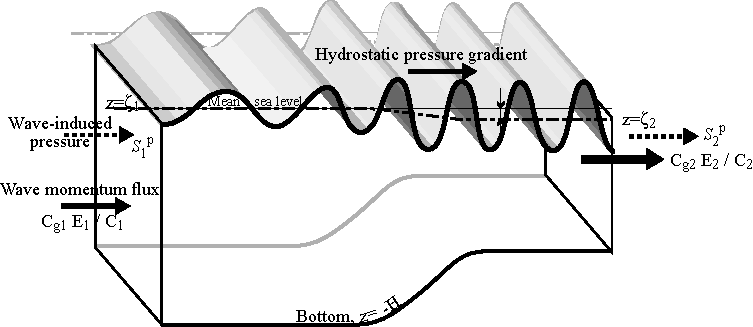
\includegraphics[width=\textwidth]{FIGS_CH_MOMENTUM/mom_flux.pdf}}
%\vspace{3.64in}
  \caption{Momentum fluxes associated to waves propagating over a variable bathymetry from left to right, towards shallower water. 
The radiation stress $S_{xx}$ 
is the sum of the flux of wave momentum $\rho_w g E C_g/C$ and the pressure correction $S^p=0.5 \rho_w g E (2 C_g/C -1)$. This 
pressure correction goes to zero in deep water. Here a difference between $S^{\mathrm{rad}}_{xx} = \rho_w g E C_g/C + S^p$ at 
points 1 and 2 drives a lowering of the mean water level from $\overline{\zeta}=\zeta_1$ to  $\overline{\zeta}=\zeta_2$. 
This phenomenon is called the set down.} 
\label{fig:mom_flux}
\end{figure}
%%%%%%%%%%%%%%%%%%%%%%%%%%%%%%%%%%%%%%%%%%%%%%%%%%%%%%%%%%%%%%%%%%%%%%%%%%%%%
This type of effect is discussed in more detail in chapter \ref{ch_littoral} which deals with nearshore 
hydrodynamics. 




